\section{Supplementary Scope}
This document accompanies \emph{CacheRAG: History-Aware Query Planning over Heterogeneous Knowledge Graph Interfaces}. It provides dataset breakdowns, additional reported results, and prompt skeletons. The main manuscript contains the stateful evaluation protocol and the comparison conditions needed to interpret its central results. This document is separate from the submission PDF.

\section{CRAG Workload Composition}
CRAG~\cite{yang2024crag} exposes KGs through five domain API families. The evaluated workload contains 578 questions, split by entity popularity into 187 head, 203 torso, and 188 tail questions. Table~\ref{tab:crag-stats} gives the domain, question-type, and timeliness breakdowns.
\begin{table}[!h]
\centering
\caption{Statistics of each question type in different question splits of CRAG.}
\label{tab:crag-stats}
\begin{tabular}{llll}
\toprule
                     & \textbf{head} & \textbf{torso} & \textbf{tail} \\
\midrule
open                 &  24  & 24   & 24   \\
finance              & 57  &  59  &  58 \\
movie                & 60  & 58   & 59  \\
music                &  7  &  31   &   7 \\
sports               &  39  &  31   &  40  \\
\midrule
simple               & 98  &  104  &  94 \\
simple\_w\_condition & 23   &  26   & 28   \\
set                  &  9  &  6   & 5   \\
comparison           &  17  & 22    & 21   \\
aggregation          & 16   & 18    & 21   \\
multi-hop            &  8  &  9   &   6 \\
post-processing      &  3   &   3   &   3  \\
false premise        &  13  & 15    & 10   \\
\midrule
real-time            & 32   &  38   &  36  \\
fast-changing        &  31  &  32   &   39 \\
slow-changing        &  22  &  27   &  19  \\
static               & 102  &  106  &  94 \\
\midrule
total               & 187 & 203 & 188 \\
\bottomrule
\end{tabular}
\end{table}

\section{Evaluation Critic}
The CRAG answer scorer is Llama-3.1-70B-Instruct. It compares responses with reference answers and labels them correct, incorrect, or missing. It is distinct from the online dispatcher, which assesses evidence without gold answers. Table~\ref{tab:auto-eval} reproduces the reported critic-agreement figures. The retained aggregate record does not specify the audit sample size or sampling procedure, so these figures should not be treated as a confidence interval or a complete validation protocol.
\begin{table}[!h]
\caption{The Auto-evaluation Accuracy of Llama-3.1 70B Instruct Model.}
\label{tab:auto-eval}
\centering
\begin{tabular}{ll}
\toprule
                    & \textbf{Llama-3.1 70B} \\
\midrule
\textbf{correct answers}     & 98.2\%        \\
\textbf{incorrect answers}   & 96.8\%        \\
\textbf{missing}             & 100\%         \\
\textbf{overall reliability} & 98.4\%       \\
\bottomrule
\end{tabular}
\end{table}

\section{Additional Results}
\subsection{Head, Torso, and Tail Questions}
Table~\ref{tab:baseline_benchmarking_crag_full} reports the existing CRAG breakdown. CacheRAG's accuracy is 0.840, 0.833, and 0.798 on head, torso, and tail questions, respectively. The table compares these results with the base language models; it does not contain a per-split comparison with every retrieval baseline.
\begin{table}[!h]
  \caption{Head/torso/tail experimental results on CRAG.}
  \label{tab:baseline_benchmarking_crag_full}
\centering
\begin{tabular}{llrrrr}
\toprule &
 \textbf{Model} & \textbf{A} & \textbf{H} & \textbf{M} & \textbf{T} \\
\midrule
head & GPT-4o   &     0.401               &             \textbf{0.086}           &    0.513               &      0.316          \\
& Llama   &   0.390                 &         0.096               &        0.513           &    0.294            \\
& Deepseek & 0.487 & 0.134 & 0.380 & 0.353 \\
\cmidrule{2-6}
& CacheRAG   &     \textbf{0.840}               &  0.123                      &   \textbf{0.037}                &     \textbf{0.717}           \\
\midrule
torso & GPT-4o   &      0.355              &                 \textbf{0.089}       &    0.557               &       0.266         \\
& Llama   &      0.305              &     \textbf{0.089}                   &        0.606           &   0.217             \\
& Deepseek & 0.394 & 0.158 & 0.448 & 0.236 \\
\cmidrule{2-6}
& CacheRAG   &     \textbf{0.833}               &     0.098                   &      \textbf{0.069}             &     \textbf{0.735}          \\
\midrule
tail & GPT-4o   &        0.266            &    0.096                    &    0.638               &       0.170        \\
& Llama   &    0.223                &          \textbf{0.053}              &       0.723            &   0.170             \\
& Deepseek & 0.319 & 0.128 & 0.553 & 0.191 \\
\cmidrule{2-6}
& CacheRAG   &     \textbf{0.798}            &    0.117                    &   \textbf{0.085}              &  \textbf{0.681}             \\
\bottomrule
\end{tabular}
\end{table}

\subsection{MMR Parameter Sensitivity}
The existing sensitivity study varies $\lambda$ over $\{0,0.25,0.5,0.75,1\}$. Figure~\ref{fig:para} reports the four CRAG metrics. Within $[0.25,1]$, accuracy changes by up to 0.7 percentage points and truthfulness by up to 0.015. The default $\lambda=0.5$ attains the highest accuracy in this sweep; the lowest hallucination rate occurs at $\lambda=0.75$.
\begin{figure*}[t]
\centering
\subfloat[Accuracy]{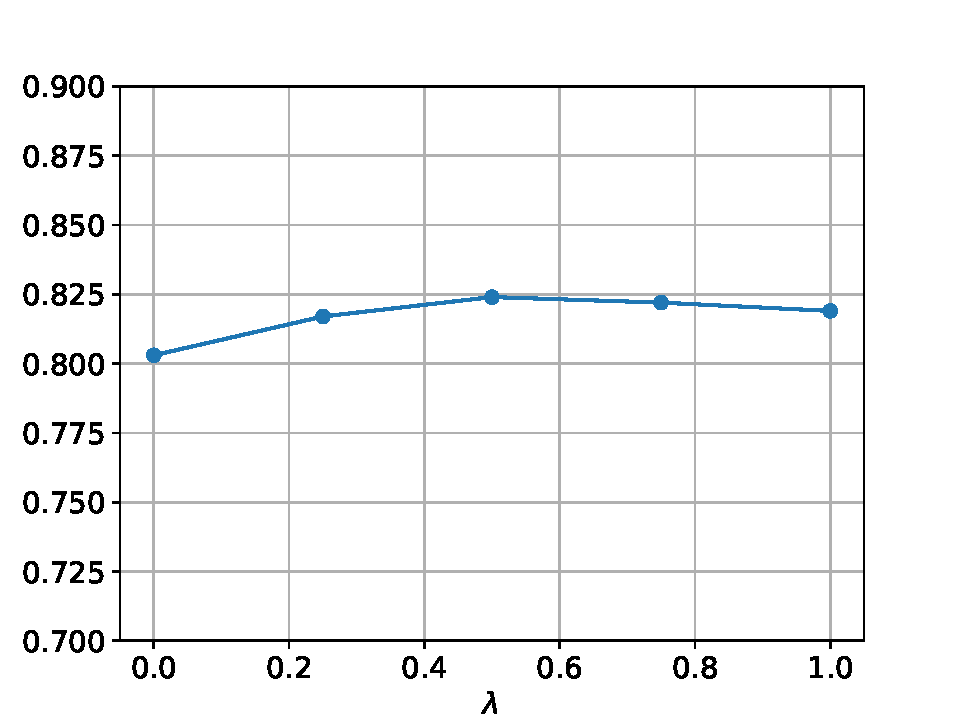
\includegraphics[width=0.24\textwidth]{figures/exp-figures/acc.pdf}}
\subfloat[Hallucination]{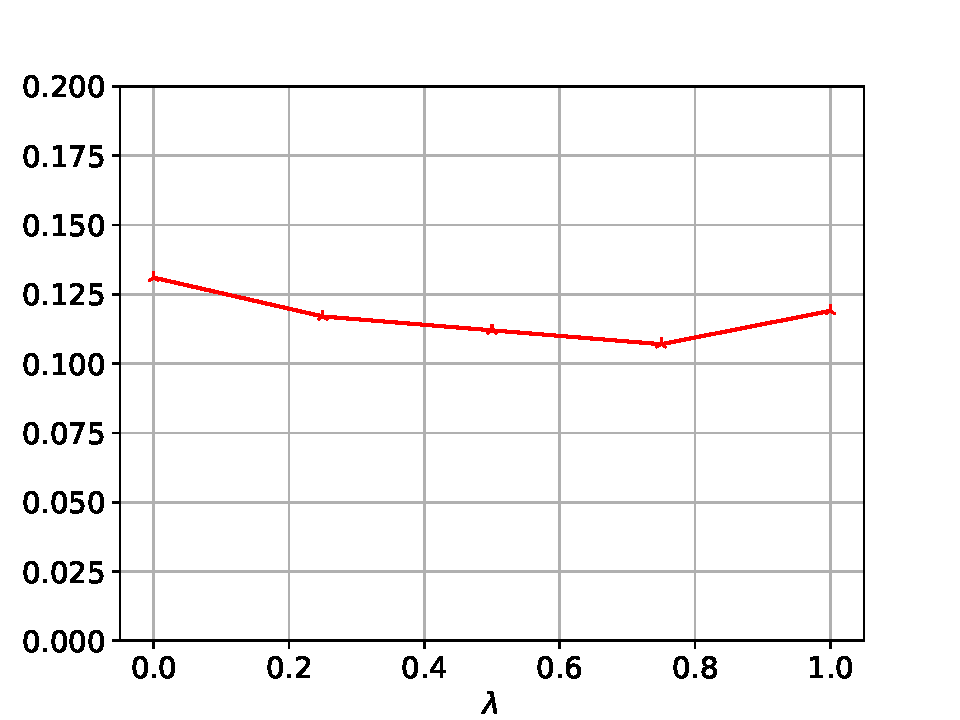
\includegraphics[width=0.24\textwidth]{figures/exp-figures/hall.pdf}}
\subfloat[Missing]{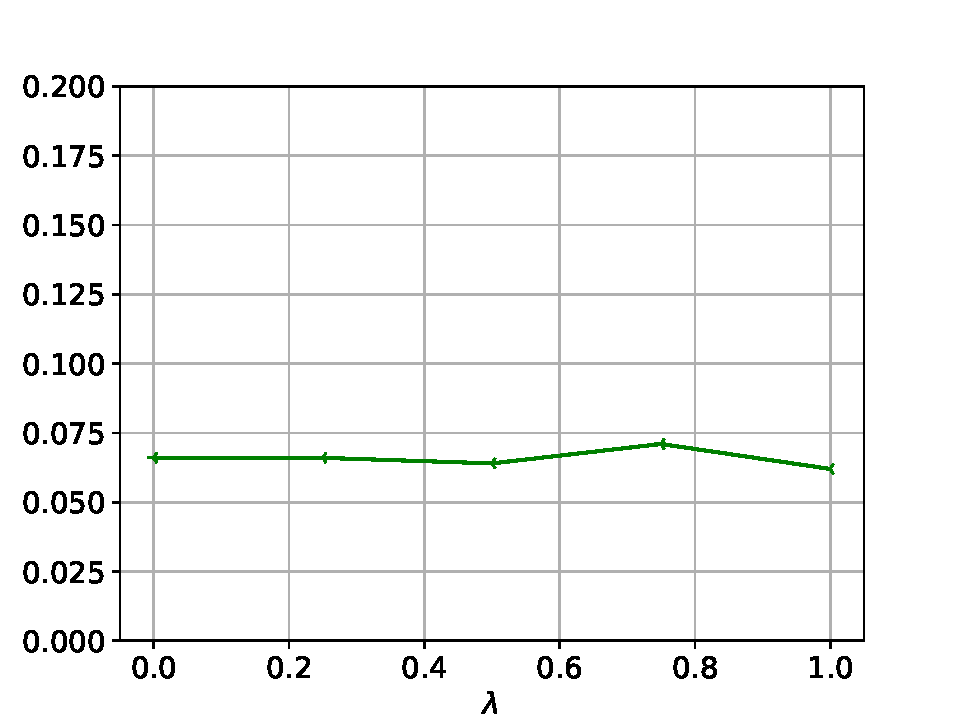
\includegraphics[width=0.24\textwidth]{figures/exp-figures/miss.pdf}}
\subfloat[Truthfulness]{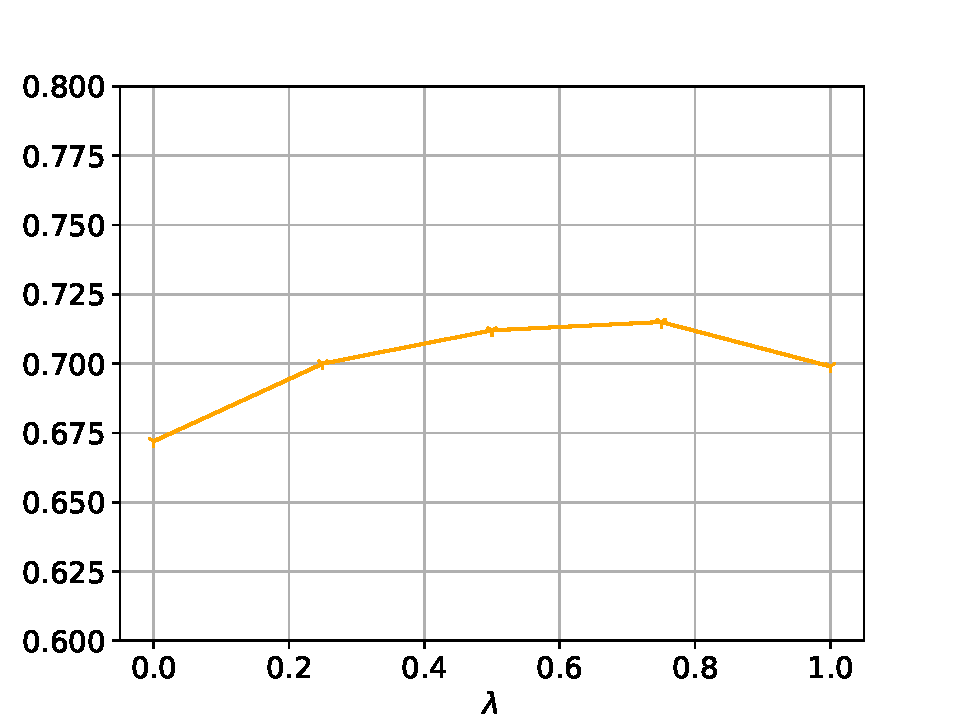
\includegraphics[width=0.24\textwidth]{figures/exp-figures/truth.pdf}}
\caption{MMR relevance--redundancy balance on CRAG.}
\label{fig:para}
\end{figure*}

\subsection{Multi-Domain Routing}
The routing comparison considers four configurations of Llama-3.1-8B-Instruct: KG names alone; names with static descriptions; static descriptions with chain-of-thought prompting; and dynamic descriptions with the same prompting. Figure~\ref{fig:domain-routing} reports the existing comparison. Dynamic descriptions update only when all calls to the selected domain API return empty/null content. This operational signal does not establish that the routing choice was wrong, and no gold domain label triggers an update.
\begin{figure}[t]
\centering
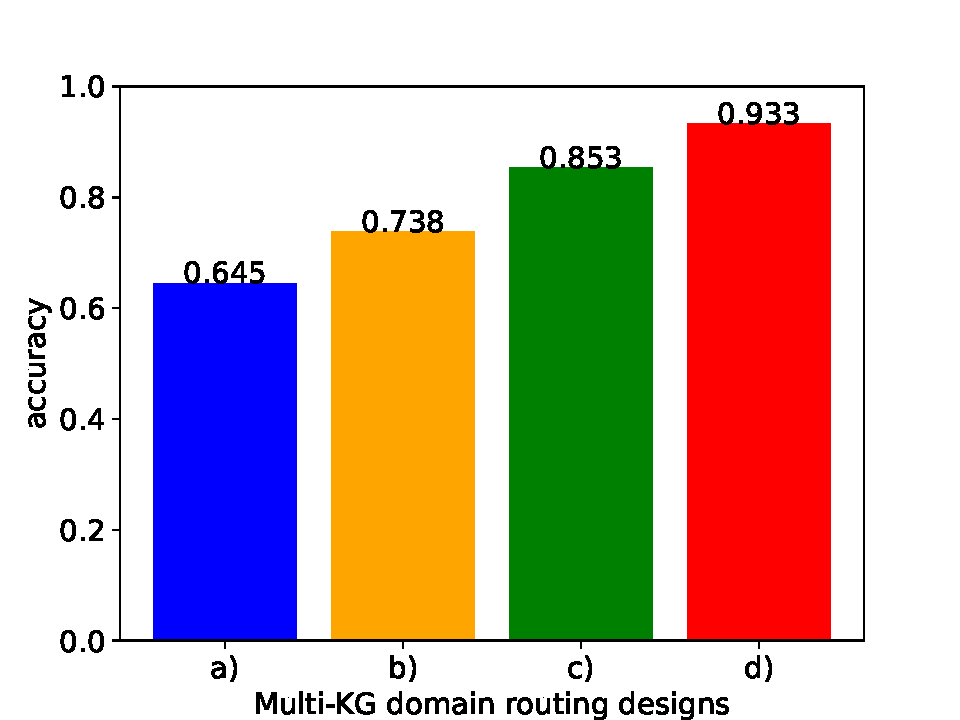
\includegraphics[width=0.98\columnwidth]{figures/multi-kg.pdf}
\caption{Reported multi-KG routing comparison. Dynamic descriptions respond to empty API content.}
\label{fig:domain-routing}
\end{figure}

\section{Prompt Skeletons and Operational Semantics}
The following are explanatory skeletons of the prompts used by the architecture. Backend-specific signature lists, schema payloads, and execution wrappers belong to the implementation configuration.

\subsection{Logical ISR Extraction}
\begin{block}{ISR extraction}
Extract the main entity and key constraints from the question. Do not generate KG predicates or schema-specific terms; use natural-language expressions from the user's question.\\
Question: [QUESTION]\\
Output:\\
Main entity: [ENTITY NAME]\\
Constraints: [NATURAL-LANGUAGE CONSTRAINTS]
\end{block}
The domain hint selects an API namespace in the multi-domain configuration. Aspect keys are normalized from the ISR constraints using backend metadata. The physical compiler then receives the ISR, local schema, and selected execution records. A prompt restriction on predicate generation is not a proof that all subsequent mappings are correct.

\subsection{Offline Question Generation}
\begin{block}{Auto-generation}
Generate reasonable natural-language questions from the provided KG triples. Generate up to five questions that people might ask. Avoid meaningless ID-based or purely numerical questions; return NA when unavoidable. Generate simple questions supported by one triple and compositional questions, such as comparison and summarization, supported by multiple triples.\\
Output: [QUESTION], [TRIPLES], [ANSWER]\\
Current triples: [SAMPLED TRIPLES]
\end{block}
Generated candidates are filtered for apparent consistency and answerability, and selected triples are compiled into executable plans. Initial cache sizes are 110 for CRAG and 48 for each SPARQL workload. Evaluation entities are excluded from sampling. The reported normalized exact-question and entity overlaps are zero; semantic and query-structure overlap are not quantified by that check.

\subsection{Domain-Description Update}
\begin{block}{Update after empty API content}
Refine the descriptions of the available KGs.\\
Current descriptions: [KG NAMES AND DESCRIPTIONS]\\
Question: [QUESTION]\\
Selected domain: [PREVIOUS DOMAIN SELECTION]\\
Previous reasoning: [PREVIOUS REASONING]\\
The selected KG API returned empty content.\\
Using this execution history, update the descriptions to better distinguish the available KGs and reduce overlapping descriptions.
\end{block}
The trigger is that all calls to the selected domain returned empty/null. The prompt receives no gold answer, gold query, or gold domain label. Descriptions persist across questions and are restored from the initial snapshot before an independent run. An example description identifies the movie API as covering films, actors, and award information, while the finance API covers stock and financial indicators. Description updates are model-generated routing context, not certified statements about backend completeness.

\begin{table*}[t]
	
	\centering
	\caption{Example initial descriptions and model-generated updated descriptions. These are routing context rather than verified backend coverage specifications.}
	\label{tab:example-domain}
	\small
\begin{tabularx}{\textwidth}{p{1.2cm}>{\raggedright\arraybackslash}X>{\raggedright\arraybackslash}X}
		\toprule
		\textbf{Domain}             & \textbf{Initial KG descriptions} & \textbf{Final KG descriptions} \\    
		\midrule
		Open & This KG includes content in Open domain. The content is based on Wikidata, you can use it as a general encyclopedia. & This KG includes general knowledge about the world, excluding specific domains like film, finance, and sports, but including information about history, science, culture, and general information about people, organizations, and events that are not related to any specific domain.\\
            Movie & This KG includes content in Movie domain. The content is based on IMDB, you can find the detailed information of the actors, movies, and oscar awards. & This KG is focused on the film industry, including information about movie titles, film scripts, and film-related events, but excluding information about music releases, financial transactions, general knowledge about the world, and sports.\\
            Music & This KG includes content in Music domain. The content is based on musicBuzz and Billboard, you can find the detailed information of the singers, albums, songs, and billboard results. & This KG is focused on the music industry, including information about musicians, music genres, album releases, and music-related events, but excluding information about film releases, financial transactions, general knowledge about the world, and sports. \\
            Finance & This KG includes content in Finance domain. The content is based on Yahoo finance, you can find the detailed information of the stock prices, eps, p/e ratio, etc. & This KG is focused on financial transactions and market trends, including economic indicators, stock market data, and financial news, with a focus on specific financial data, such as stock prices, financial reports, and market analysis.\\
            Sports & This KG includes content in Sports domain. The content is based on basketball and soccer, you can find the detailed information of the NBA and Premier League match results and team leaders. & This KG is focused on the competitive aspects of sports, including information about teams, players, championships, and tournaments, as well as the rules, strategies, and techniques of specific sports.\\
		\bottomrule
	\end{tabularx}
\end{table*}

\section{Cost Interpretation}
The main manuscript separates cache retrieval cost from graph execution cost. With incremental redundancy scores, selecting $k$ records from $b$ candidates requires $O(kb)$ similarity evaluations, plus text-processing costs. The default cache grows with admitted records. The LRU variant caps each leaf bucket at ten records, but domain fallback can combine several buckets.

The breadth parameter retains at most 30 predicates, while a selected predicate can have many values. Candidate enumeration may inspect more triples than are retained. Therefore, limits on traversal rounds and predicate count alone do not establish a constant bound on total memory, response bytes, or backend work. The synthetic point/star-query study concerns indexed retrieval over 40,000--1.28 million triples and does not measure a universal end-to-end scaling law.

\section{Reproduction Context}
The reported main model is DeepSeek-V3-0324, with a Llama-3.1-8B-Instruct CRAG router, a task-specific off-the-shelf parser for the full SPARQL variant, BM25 MMR with $\lambda=0.5$ and $k=5$, and DPR predicate ranking with a top-30 limit. The main manuscript states initial-state sizes, admission and router-update signals, persistence, reset rules, and matched comparison conditions. Full reproduction additionally depends on the exact initial snapshots, workload order, backend snapshots, prompts, model-serving settings, and evaluation scripts supplied with an implementation artifact.
